\chapter{Review of Development Tools } \label{chap:tools}

\section{The Nao humanoid robot}

The robot available for the research is a Nao v5.0. The Nao is a humanoid robot, designed purposely to look approachable, which has been developed by Aldebaran-Robotics with the objectives of being affordable without sacrificing quality and performance \cite{gouaillier2008nao}. Indeed it brings access to an affordable (under 5K Euros) and performant biped robot to research laboratories and the mass market \cite{shamsuddin2011humanoid}, with 25 degrees of freedom, two cameras, speech capabilities and the ability to autonomously execute a range of tasks. Figure \ref{fig:nao_robot} illustrates the features of the Nao, including the 6 degrees of freedom in the arm: 2 at the shoulder, 2 at the elbow, 1 at the wrist and 1 for the hands grasping (open/closed) \cite{gouaillier2008nao}.

\begin{figure}[h!]
        \centering
        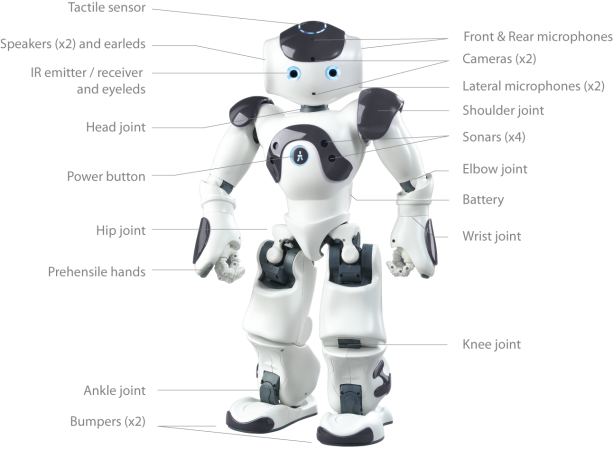
\includegraphics[width=0.5\textwidth]{figures/naoRobot.png}
        \caption{Nao features for v5.0 version \cite{aldebaran}.}
        \label{fig:nao_robot}
\end{figure}

\section{The NaoQI API}

NaoQi is the API provided by Aldebaran-Robotics to interface with the Nao. It is a modular
framework which can cope with a range of binaries developed in different languages, allowing
for a distributed environment which may be partly or wholly deployed on the robot \cite{gouaillier2008nao}. The level of abstraction available from the API includes execution of high-level autonomous behaviours such as causing the gaze of the robot to follow a ball, causing the robot to walk to a position, and causing the robot to stand after having fallen; and lower-level behaviours such as setting the joint values of the robot. A feature which is not present in the API, however, is an appropriate method for maintaining the robot’s relationship with other objects in the world, such as a tablet or a camera. For managing such information, the Robot Operating System has been employed.

\section{The Robot Operating System (ROS)}

Recognising that the required breadth of expertise for implementing software for a robotics
project is typically well beyond the capabilities of a single researcher, the Robot Operating
System (ROS) was developed to support large-scale software integration efforts \cite{quigley2009ros}. Its design criteria are listed as being peer-to-peer: allowing multiple hosts to be connected in a heterogeneous network rather than centralized to avoid unnecessary traffic flow; tools-based: where
small tools exist in different modules, arguably compensating for the loss in efficiency with the
gains in stability and complexity management; multilingual: where language-neutral messaging processing between modules allows mixing of different coding languages inside the modules and Free and Open-Source: with the full source code being made publicly available to facilitate the parallel design and debugging of different levels of the software \cite{quigley2009ros}.


\subsection{Framework}
In the ROS framework, nodes represent software modules, which communicate with each other
through messages over topics. Nodes should subscribe to relevant topics which they are interested in receiving messages over: a message can carry an arbitrary amount of data, structured into different fields (including, for example, arrays of other message types), and multiple nodes may be simultaneously publishing. Nodes can be connected to each other in a graph-like manner: the resulting graph may be arbitrarily complex, involving cycles, one-to-many or many-to-many connections. If a synchronous transaction is a more appropriate method of communication than the broadcasting exhibited by topics, a service may be used instead which has a defined request and response message format.

\subsection{Benefits}
In addition to those previously mentioned, the benefits of using ROS for robotics development
include that:
\begin{itemize}
\item Nodes may disconnect and reconnect to the network at run-time, allowing for ease in
debugging/prototyping of an experimental node amongst an existing framework of well-
debugged nodes by not requiring that they restart on changes to the node being developed.
\item Messages published can be logged for playback at a different time, without the need for
the nodes originally publishing the messages to be running. This is useful for software
development in research, where it is not desirable to connect all sensors to the system for
every test. In the case of interaction experiments, the messages may simulate the input
from a user interacting with the system which was captured in a once-off opportunity, for
offline analysis. ROS bags has been the perfect complement for the data recording.
\item Different frames of reference in a system, such as the position of grippers on a robot or an
object detected in space by a camera on the robot, can be related to each other through
a transformation tree which is generated dynamically by the tf transformation library. The ease of computing a transformation between two frames without needing to be concerned with the intermediate frames. Therefore, steps have been taken to continue using The ROS framework to interface with Nao 
\footnote{http://wiki.ros.org/nao\_robot} ). 
\end{itemize}

\section{The OpenCV library}
OpenCV\footnote{http://opencv.org} (open source computer vision) is the most popular open source library for Computer Vision related applications up to now, spanning from many very basic tasks like capture and pre-processing of image data, but also to high-level algorithms such as feature extraction, motion tracking or machine learning. It is released under a BSD license and hence it’s free for both academic and commercial use. It has C++, C, Python and Java interfaces and supports Ubuntu Linux. OpenCV was designed for computational efficiency and with a strong focus on real-time applications, fact that makes it perfect for the work presented in this document.

\section{The dlib library}
Dlib\footnote{http://dlib.net} is a general purpose cross-platform C++ library designed using contract programming and modern C++ techniques (including support for the most recent compilers). It is open source software and licensed under the BSD license. The most valuable asset that brings to the project is a robust real-time 2D face pose estimation, including features like; eyes, mouth, nose and eyebrows among others. The fact that it allow us to track precisely, even with occlusions or in poor light conditions, the face of the user in a range from $ -45\degree $  till $ 45\degree $ makes it suitable for this work. In addition, the library allows a flexible integration with OpenCV, through several methods for matrix and point conversions between both libraries. For these reasons, it has been used to track children's faces and features extraction.